% !TEX encoding = UTF-8 Unicode

\section{Sensorenhet}

Sensorenheten är den enhet som behandlar all sensordata. Den samlar in data från 
avståndssensorerna och linjesensorerna som den sedan antingen omvandlar till 
cm värden i avståndsensorns fall, eller trösklar och ger diskreta varierande storheter 
som i linjesensorns fall. Linje sensorn kommunicerar sedan med kommunikationsenheten
som förmedlar värdena till styrenheten och till PCn.

\subsection{Hårdvara}

\begin{figure}[H]
  \centering
 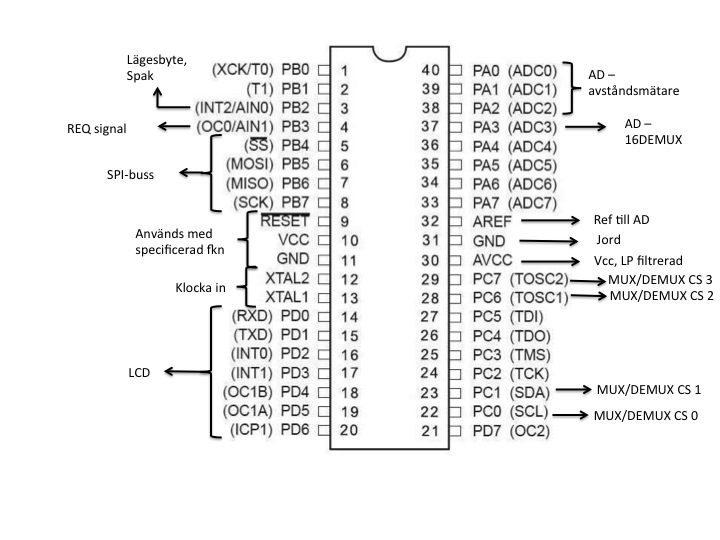
\includegraphics[angle=0,scale=0.5]{bilder/PIN_sensor.jpg}
  \caption{Sensorsenhetens pin-anslutningar}
  \label{fig:PINsensor}
\end{figure}

\subsubsection{Linjeföljarsensor}
För att maximera robotens framförhållning är sensorerna monterade framför roboten 
så långt fram som möjligt ca 3 mm ovanför marken. Linjesensorn består av 11st lysdioder 
med 11st ljuskänsliga transistorer, en multiplex och en demultiplex.

\begin{figure}[H]
  \centering
 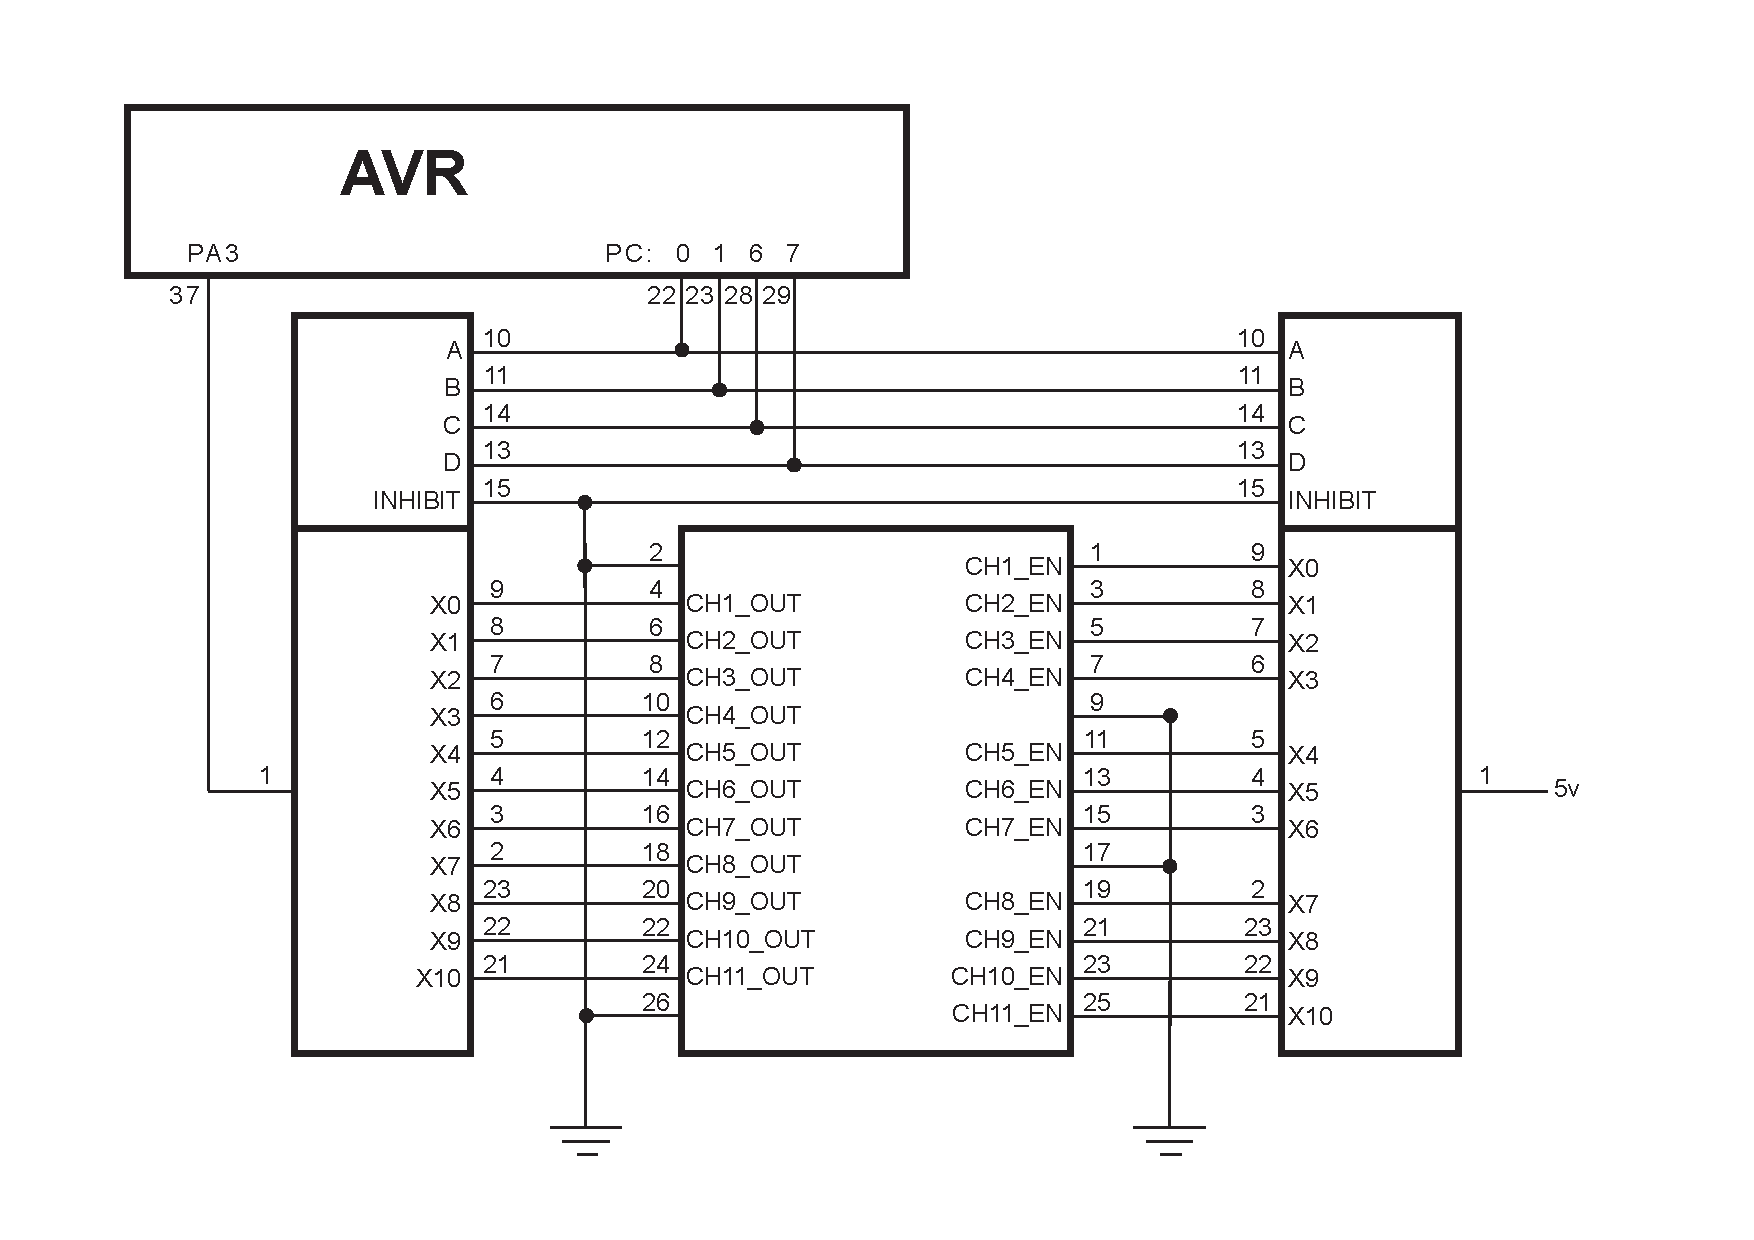
\includegraphics[angle=0,scale=0.5]{bilder/Uppkoppling_linjesensorer.pdf}
  \caption{Uppkoppling linjesensorer}
  \label{fig:Uppkoppling_linjesensorer}
\end{figure}

CH1 EN - CH11 EN är ingångar som leder signalen (logiskt ) vidare till lysdioderna. 
CH1  OUT - CH11 OUT Leder svarssignalen från transistorerna vidare mot styrenhetens 
AVR. Multiplexen och demultiplexen styrs med signalerna A - D från AVRen. Inhibit 
signalen är jordad då dataväljning alltid ska vara tillåten.



\subsubsection{Upptäckning av riktningsmarkeringar}
\label{sec:riktmark}
Då roboten är i en labyrint kommer linjeföljarsensorn huvudsakligen användas 
för att hitta riktningsmarkeringar. Dessa markeringar används för att visa i 
vilken riktning roboten ska färdas i nästkommande korsning.  I enlighet med 
banspecifikationen, se *REF BANSPEC*, är funktionen anpassad för att uppfatta 
följande signaler:

Högersväng visas med en tunn tejpmarkering följd av en tre gånger så tjock.
Vänstersväng visas genom en tjock tejpmarkering följd av en tre gånger så tunn.
Framåt visas genom två tunna tejpmarkeringar.

Vid varje uppdatering av samtliga linjeföljarsensorer görs en kontroll om de 
tre mittersta sensorerna ligger över tejp. Är så fallet så börjar antalet 
gånger linjesensorerna uppdateras att räknas. När de tre mittersta sensorerna 
inte längre ligger över tejp sparas antalet iterationer som sensorerna 
tillbringat över tejpen. Proceduren upprepas därefter och antalet iterationer 
jämförs för att se vilken tejpbit som var bredast, den första eller den andra
. Resultatet sparas därefter och efterfrågat kommando utförs i nästkommande 
korsning, se \ref{sec:upptackkorsning}.


\subsubsection{Avståndssensorer}

\subsubsection{Upptäckning av korsningar och 90\degree svängar}
\label{sec:upptackkorsning}
Enligt specifikationen av den bana som roboten ska kunna följa, framgår det 
att det före alla korsningar ska finnas tejpmarkeringar som visar i vilken 
riktning roboten ska svänga, se \ref{sec:riktmark}. Roboten kommer att 
upptäcka korsningar om två av riktningarna höger, vänster och framåt visar 
mer än 80 cm.

Roboten kommer att upptäcka 90\degree svängar om det är längre än 80 cm åt 
höger eller vänster(inte båda), samt mindre än 35cm framåt.

Upptäcker roboten en korsning kommer det kommando som beskrivits av tidigare 
tejpmarkeringar att skickas till styrenheten. Datat som skickas är skrivet 
för att uppfattas som ett så kallat specialkommando, det vill säga 
styrenheten har en procedur som utförs utan att ta hänsyn till den reglerdata 
som skickas från sensorenheten. Märk att detta specialkommando innehåller en 
framkörning till mitten av korsningen, till skillnad från 90\degree svängar 
som utförs omedelbart.

Upptäcker korsningen en 90\degree sväng kommer ett annat specialkommando att 
utföras, där roboten svänger 90\degree åt det håll som avståndssensorerna 
visar har det längre avståndet.


\subsubsection{Display}
Robotens display-enhet är av typ \emph{LCD JM162A}. Displayen används för att visa avståndssensorernas värden. Eftersom sensorerna bara kan ge korrekta värden i intervallet 20-120 cm så kommer även displayen arbeta i detta intervall. Displayen arbetar i åtta databitarsläge och visar två rader med tecken. 

%Pinnar
Förutom de åtta databitarna som överförs för varje tecken till displayen så går ytterligare två signaler mellan sensorenhetens mikroprocessor och displayenheten: \emph{Enable} och \emph{Register select}. Enable-signalen signalerar till displayen att något ska skrivas ut, och Register select väljer mellan input-lägena 'data' och 'function'. Då det aldrig är någon data som läses från displayen så är pinnen \emph{R/W} konstant låg. 

%Kod
Sensorenheten har två funktioner som kan kallas för att skriva ut ett tecken på displayen. I funktionen \emph{char\_to\_display} anges parmetrarna vilket tecken (givet i ASCII-kod) som ska skrivas ut, samt vilken position på displayen som ska skrivas till. Denna funktion används för bokstäver. För att skriva ut sensorvärden används funktionen \emph{data\_to\_display}, vilken tar parametrarna för sensorvärdet i cm samt vilken sensor som skickat det. 

Sensorprocessorn har också en funktion för att konvertera cm-värdet till ASCII-kod, vilken används av \emph{data\_to\_display}.

\subsection{Mjukvara}

\subsubsection{AD}

\subsubsection{Linjesensor}


\subsubsection{Avståndsberäkning}


\subsubsection{Kommunikation}

